\documentclass[10pt]{article}
\usepackage[margin=1in]{geometry}
\usepackage{amsmath,amsthm,amssymb}
\usepackage{mathtools,bbm}
\usepackage{graphicx}
\usepackage{subcaption}
\usepackage{algorithmicx}
\usepackage{algorithm}
\usepackage{algpseudocode}
\usepackage[colorlinks,linkcolor=blue]{hyperref}
\usepackage[noabbrev]{cleveref}
\usepackage{courier}
\usepackage{enumitem}
\usepackage[parfill]{parskip}
\usepackage{multicol}
\usepackage{listings}
\usepackage{color}
\usepackage{xcolor}



\setlist[itemize]{itemsep=.01cm, topsep=.01cm}
\setlist[enumerate]{itemsep=.01cm, topsep=.01cm}


\oddsidemargin 0in
\evensidemargin 0in
\textwidth 6.5in
\topmargin -0.5in
\textheight 9.0in
\setlength{\parskip}{8pt}

\newcommand{\head}[4]{
\thispagestyle{plain}
\newpage
\setcounter{page}{1}
\noindent
\begin{center}
\framebox{ \vbox{ \hbox to 6.28in
{CIS 4190/5190: Applied Machine Learning \hfill #1}
\vspace{4mm}
\hbox to 6.28in{\hfill \large\bf #2 \hfill}% % centered title
\vspace{4mm}
\hbox to 6.28in
{{\it #3 \hfill #4}}
}}
\end{center}
}


\begin{document}
\head{Spring 2026}{News Source Classification from Headlines}{Team Members: Isaac Dcruz, Arjun Verma, Maxwell Zhang}{Project: News Source}

\textbf{Code:} \href{https://github.com/Maxwell938623/news-source-classification}{\texttt{github.com/Maxwell938623/news-source-classification}}\\
\textbf{Dataset:} \href{https://huggingface.co/datasets/Maxwell938623/foxnews-nbc-headlines}{\texttt{huggingface.co/datasets/Maxwell938623/foxnews-nbc-headlines}}\quad\emph{(\textcolor{red}{TODO: replace with final HF dataset URL after \texttt{push\_to\_hub})}}

\section{Introduction}
In this project, we built an end-to-end binary NLP classification pipeline to predict whether a headline came from Fox News or NBC News. Our core objective was to make the system reproducible and extensible: every major stage (URL collection, scraping, preprocessing, splitting, training, evaluation, and prediction) is implemented as a script with explicit inputs/outputs and logs.

We first reproduced the handout baseline (\texttt{TF-IDF(max\_features=100) + LogisticRegression(max\_iter=100)}), then expanded to a controlled experiment framework covering multiple feature/model families. Our training framework evaluates a large configuration space and selects the best model by validation macro-F1 before retraining on train+validation and evaluating once on the held-out test set.

This report reflects the current repository state and includes finalized implementation details and experimental outcomes produced in our latest run cycle.

\section{Core Components}

\subsection{Data Collection and Dataset}
Our data pipeline follows a two-stage collection process designed to maximize coverage while keeping source labels reliable. First, we discover article URLs using \texttt{src/collect\_urls.py}. This script traverses robots-discovered sitemap indexes, configured sitemap seeds, RSS/Atom feeds, and section pages for FoxNews and NBC domains. We use this broad discovery strategy because a single source (for example, only one sitemap) misses many valid article pages, especially for historical coverage.

Second, we scrape headline text with \texttt{src/scrape.py}. The scraper fetches each URL with retry/backoff logic and then applies a robust extraction cascade so that template variation across pages does not cause widespread failures:
\begin{enumerate}
    \item source-specific \texttt{h1} class heuristics,
    \item \texttt{itemprop=headline},
    \item first generic \texttt{h1},
    \item \texttt{og:title},
    \item fallback \texttt{title}.
\end{enumerate}

At the raw-data stage, our repository contains 172,488 discovered URLs (115,266 FoxNews; 57,222 NBC) and 132,271 scraped article rows across the two source-specific files (Fox: 82,126 successes / 2,699 fetch failures; NBC: 47,205 successes / 241 fetch failures).

We then consolidate and preprocess using \texttt{src/preprocess.py}. The preprocessing stage enforces quality and leakage controls by applying scrape-status filtering, null/empty removal, HTML unescaping/tag stripping, whitespace normalization, within-source deduplication, cross-source duplicate removal, and label validation. In addition to the canonical cleaned text, we generate multiple preprocessing variants to support fair ablation studies:
\texttt{headline\_minimal}, \texttt{headline\_lowercase}, \texttt{headline\_nopunct}, \texttt{headline\_nostop}, \texttt{headline\_lemma}.

For internal evaluation, we use \texttt{src/split.py} to produce stratified 70/15/15 train/val/test splits with fixed seed 42 and store split metadata for reproducibility. The final processed dataset contains 128,861 headlines (Fox 81,837 / NBC 47,024) with stratified splits (train: 90,202; val: 19,329; test: 19,330). We also identified 7,940 very short headlines (\textless 3 words). Instead of dropping these automatically, we retain them and account for their behavior in error analysis, since short headlines are a meaningful real-world edge case.

\subsection{Model Design}
We designed model development as a staged but fully scripted process from baseline reproduction to representation-rich and ensemble architectures. All model files in \texttt{src/models} share the same training contract through \texttt{src/models/\_base.py}: each \texttt{ModelConfig} specifies \texttt{name}, \texttt{prep\_col}, and an unfitted sklearn estimator; the runner trains on \texttt{train.csv}, ranks by validation macro-F1, retrains the selected configuration on train+val, and evaluates exactly once on held-out test. This standardized protocol ensures direct comparability across families.

\textbf{Global training/evaluation protocol (applies to every classical family):}
\begin{itemize}
    \item Fixed label encoding (\texttt{FoxNews=0}, \texttt{NBC=1}) and fixed split seed (42).
    \item Selection metric: validation macro-F1 (\texttt{val\_f1\_macro}).
    \item Final reporting metrics: accuracy, macro/weighted F1, per-class F1, macro precision/recall, confusion matrix.
    \item Refit policy: winner retrained on train+val before single test evaluation.
    \item Artifact policy: save model (\texttt{models/*\_best.joblib}) and metadata JSON with winning config and test metrics.
\end{itemize}

\textbf{Baseline model (\texttt{src/train\_baseline.py}):}
\begin{itemize}
    \item Handout-consistent baseline: \texttt{TfidfVectorizer(max\_features=100)} + \texttt{LogisticRegression(max\_iter=100)}.
    \item Used as a low-capacity anchor to quantify absolute gains from richer representations and stronger learners.
\end{itemize}

\textbf{Classical model families (all implemented and executed):}
\begin{enumerate}
    \item \textbf{Word TF-IDF + Logistic Regression (\texttt{tfidf\_logreg.py}, 25 configs).}
    We sweep vocabulary size (\texttt{max\_features} from 100 to 20,000), word n-gram ranges \((1,1)\), \((1,2)\), \((1,3)\), \((2,2)\), regularization strength \(C\in\{0.01,\dots,20\}\), and preprocessing variants (\texttt{minimal/lowercase/nopunct/nostop/lemma}). All variants use \texttt{sublinear\_tf=True}; stopword handling is adjusted to avoid confounding in already de-stopped columns.

    \item \textbf{Word TF-IDF + LinearSVC (\texttt{tfidf\_svm.py}, 22 configs).}
    We evaluate large-margin linear SVMs on sparse TF-IDF with sweeps over \(C\), \texttt{max\_features}, and n-gram ranges. Because raw \texttt{LinearSVC} has no probability output, calibrated variants (\texttt{CalibratedClassifierCV}, sigmoid/Platt scaling, CV=3) are included for downstream soft-voting/stacking compatibility.

    \item \textbf{Word TF-IDF + MultinomialNB (\texttt{tfidf\_nb.py}, 22 configs).}
    We sweep smoothing \(\alpha\), feature counts, n-gram ranges, and preprocessing variants. Critically, all NB pipelines set \texttt{norm=None} in TF-IDF to preserve count-like magnitude semantics required by multinomial likelihood modeling.

    \item \textbf{Character n-gram models (\texttt{char\_ngram.py}, 24 configs).}
    We use \texttt{analyzer=char\_wb} (token-boundary-aware character n-grams) with LR/SVM, ranges such as \((2,4)\) to \((5,7)\), and feature-count sweeps up to 20,000. We explicitly test capitalization-preserving input (\texttt{headline\_minimal}) vs lowercased input, and include combined word+char \texttt{FeatureUnion} pipelines to exploit complementary lexical and orthographic cues.

    \item \textbf{Stylometric tabular models (\texttt{stylometric.py}, 12 configs).}
    We extract 15 handcrafted headline-style features (e.g., length statistics, punctuation frequencies, capitalization ratios, digit ratio, title-case ratio) and train LR, LinearSVC, RandomForest, and HistGradientBoosting variants. This family isolates writing-style signal independent of specific vocabulary identity.

    \item \textbf{Hybrid sparse unions (\texttt{hybrid.py}, 10 configs).}
    We combine word TF-IDF, optional char TF-IDF, and stylometric features through \texttt{FeatureUnion}, using \texttt{SparseWrapper} to keep stylometric outputs CSR-compatible. A \texttt{MaxAbsScaler} is applied before the classifier so low-magnitude style features are not drowned out by high-dimensional TF-IDF coordinates.

    \item \textbf{Soft-voting ensembles (\texttt{voting\_ensemble.py}, 7 configs).}
    We average class probabilities from diverse base learners (word LR, char LR, MNB, calibrated SVM, stylometric LR), including weighted voting (\([2,1,1]\)) and feature-diverse branches. Minimal-input variants preserve capitalization for stylometric usefulness while normalizing TF-IDF branches as needed.

    \item \textbf{Stacking ensembles (\texttt{stacking\_ensemble.py}, 7 configs).}
    We train meta-learners on out-of-fold base-model probabilities (\texttt{stack\_method='predict\_proba'}) with CV=5 (or CV=3 for the heaviest 5-base stack). Meta-learners include LR and HistGradientBoosting; base learners include LR, char models, MNB, calibrated SVM, and stylometric branches depending on configuration.
\end{enumerate}

Across these eight classical families we execute \(25+22+22+24+12+10+7+7=129\) configurations, matching the full classical sweep reported in this project cycle.

\textbf{Transformer baselines (\texttt{src/train\_modernbert.py}):}
\begin{itemize}
    \item DistilBERT (\texttt{distilbert-base-uncased}) and DeBERTa-v3-small (\texttt{microsoft/deberta-v3-small}) are evaluated on subsampled CPU runs as compute-constrained references for the broader transformer family.
    \item ModernBERT-base (\texttt{answerdotai/ModernBERT-base}, 149M params) is fine-tuned on the full 90,202 / 19,329 / 19,330 split with Hugging Face \texttt{Trainer} on Apple Silicon (MPS), batch=32, max\_len=64, lr=2e-5, weight decay=0.01, warmup ratio=0.06, 3 epochs, best-checkpoint selection by validation macro-F1, fixed seed 42. ModernBERT (Dec 2024, Answer.AI/LightOn) is the current SOTA-class encoder for short-text classification and was selected as our strong-model reference for May 2026.
    \item These runs provide a compute-aware SOTA reference against the strongest classical pipeline on the same task formulation.
\end{itemize}

\subsection{Evaluation and Model Performance}
Our evaluation stack is implemented at three levels. First, \texttt{train\_baseline.py} provides exact baseline reproduction metrics and feature inspection. Second, \texttt{train\_best\_model.py} and family-specific runners produce full experiment tables, selection metadata, and best-model metrics/plots under a common selection protocol. Third, \texttt{evaluate.py} supports deeper post-hoc diagnostics including misclassified samples, confidence-ranked errors, and headline-length error trends.

Concretely, the tooling exports:
\begin{itemize}
    \item scalar metrics (accuracy, macro-F1, per-class F1, precision/recall),
    \item confusion matrices,
    \item ROC AUC and ROC curves from probability/score outputs,
    \item model comparison plots,
    \item feature analyses where supported by model type,
    \item error-analysis artifacts for qualitative review.
\end{itemize}

\textbf{Final reported metrics:}
\begin{itemize}
    \item Baseline test metrics (completed): accuracy = 0.7051, macro-F1 = 0.6481, FoxNews F1 = 0.7897, NBC F1 = 0.5066.
    \item Best classical model (completed): \texttt{HYB\_word12\_char36\_mf5000\_style\_LR}, validation macro-F1 = 0.8296, test accuracy = 0.8420, test macro-F1 = 0.8294, FoxNews F1 = 0.8758, NBC F1 = 0.7829.
    \item \textbf{Best overall model (completed): ModernBERT-base (\texttt{answerdotai/ModernBERT-base}), validation macro-F1 = 0.8918, test accuracy = 0.8956, test macro-F1 = 0.8872, FoxNews F1 = 0.9180, NBC F1 = 0.8564 (full 90{,}202 / 19{,}329 / 19{,}330 split, 3 epochs, MPS, training time $\approx$ 33 min).}
    \item Model comparison figures (completed): \texttt{baseline\_confusion\_matrix.png}, \texttt{best\_confusion\_matrix.png}, \texttt{experiment\_comparison.png}, and \texttt{modernbert\_confusion\_matrix.png}.
\end{itemize}

Relative to baseline, our best classical model improves test accuracy by approximately 13.7 percentage points (0.7051 $\rightarrow$ 0.8420) and macro-F1 by approximately 18.1 points (0.6481 $\rightarrow$ 0.8294). The fine-tuned ModernBERT-base improves further: $+19.0$ points test accuracy (0.7051 $\rightarrow$ 0.8956) and $+23.9$ points macro-F1 (0.6481 $\rightarrow$ 0.8872) over baseline, and $+5.4$ accuracy / $+5.8$ macro-F1 over the strongest classical hybrid. The largest gain comes on the minority class (NBC F1 0.7829 $\rightarrow$ 0.8564, $+7.4$), indicating that contextual representations generalise better than sparse n-gram + stylometric features when the headline lacks unambiguous source-specific lexical cues.

We executed every standalone training entry point under \texttt{src/models} (\texttt{tfidf\_logreg.py}, \texttt{tfidf\_svm.py}, \texttt{tfidf\_nb.py}, \texttt{char\_ngram.py}, \texttt{stylometric.py}, \texttt{hybrid.py}, \texttt{voting\_ensemble.py}, \texttt{stacking\_ensemble.py}) and report each family's best test-set metrics in Table~\ref{tab:results}.

\begin{table}[h]
\centering
\small
\begin{tabular}{lccc}
\hline
Model & Accuracy & Macro-F1 & ROC AUC \\
\hline
baseline & 0.7051 & 0.6481 & 0.7194 \\
tfidf\_logreg\_best & 0.8014 & 0.7812 & 0.8779 \\
tfidf\_svm\_best & 0.8133 & 0.7973 & 0.8870 \\
tfidf\_nb\_best & 0.7740 & 0.7669 & 0.8530 \\
char\_ngram\_best & 0.8303 & 0.8146 & 0.9079 \\
stylometric\_best & 0.7457 & 0.7295 & 0.8229 \\
hybrid\_best & 0.8420 & 0.8294 & 0.9202 \\
voting\_ensemble\_best & 0.8124 & 0.8014 & 0.8909 \\
stacking\_ensemble\_best & 0.8282 & 0.8162 & 0.9085 \\
distilbert (CPU, 10k subsample, 1 epoch) & 0.8058 & 0.7948 & 0.8862 \\
deberta\_v3\_small (CPU, 5k subsample, 1 epoch) & 0.8024 & 0.7931 & 0.8869 \\
\textbf{modernbert\_base (MPS, full split, 3 epochs)} & \textbf{0.8956} & \textbf{0.8872} & --- \\
\hline
\end{tabular}
\caption{Held-out test performance for all model families and transformer baselines. ModernBERT-base is the overall best model; ROC AUC for the transformer is omitted as the per-instance probability outputs are reported separately in \texttt{reports/metrics\_modernbert\_base.json}.}
\label{tab:results}
\end{table}

\begin{figure}[h]
\centering
\begin{subfigure}[t]{0.62\textwidth}
\centering
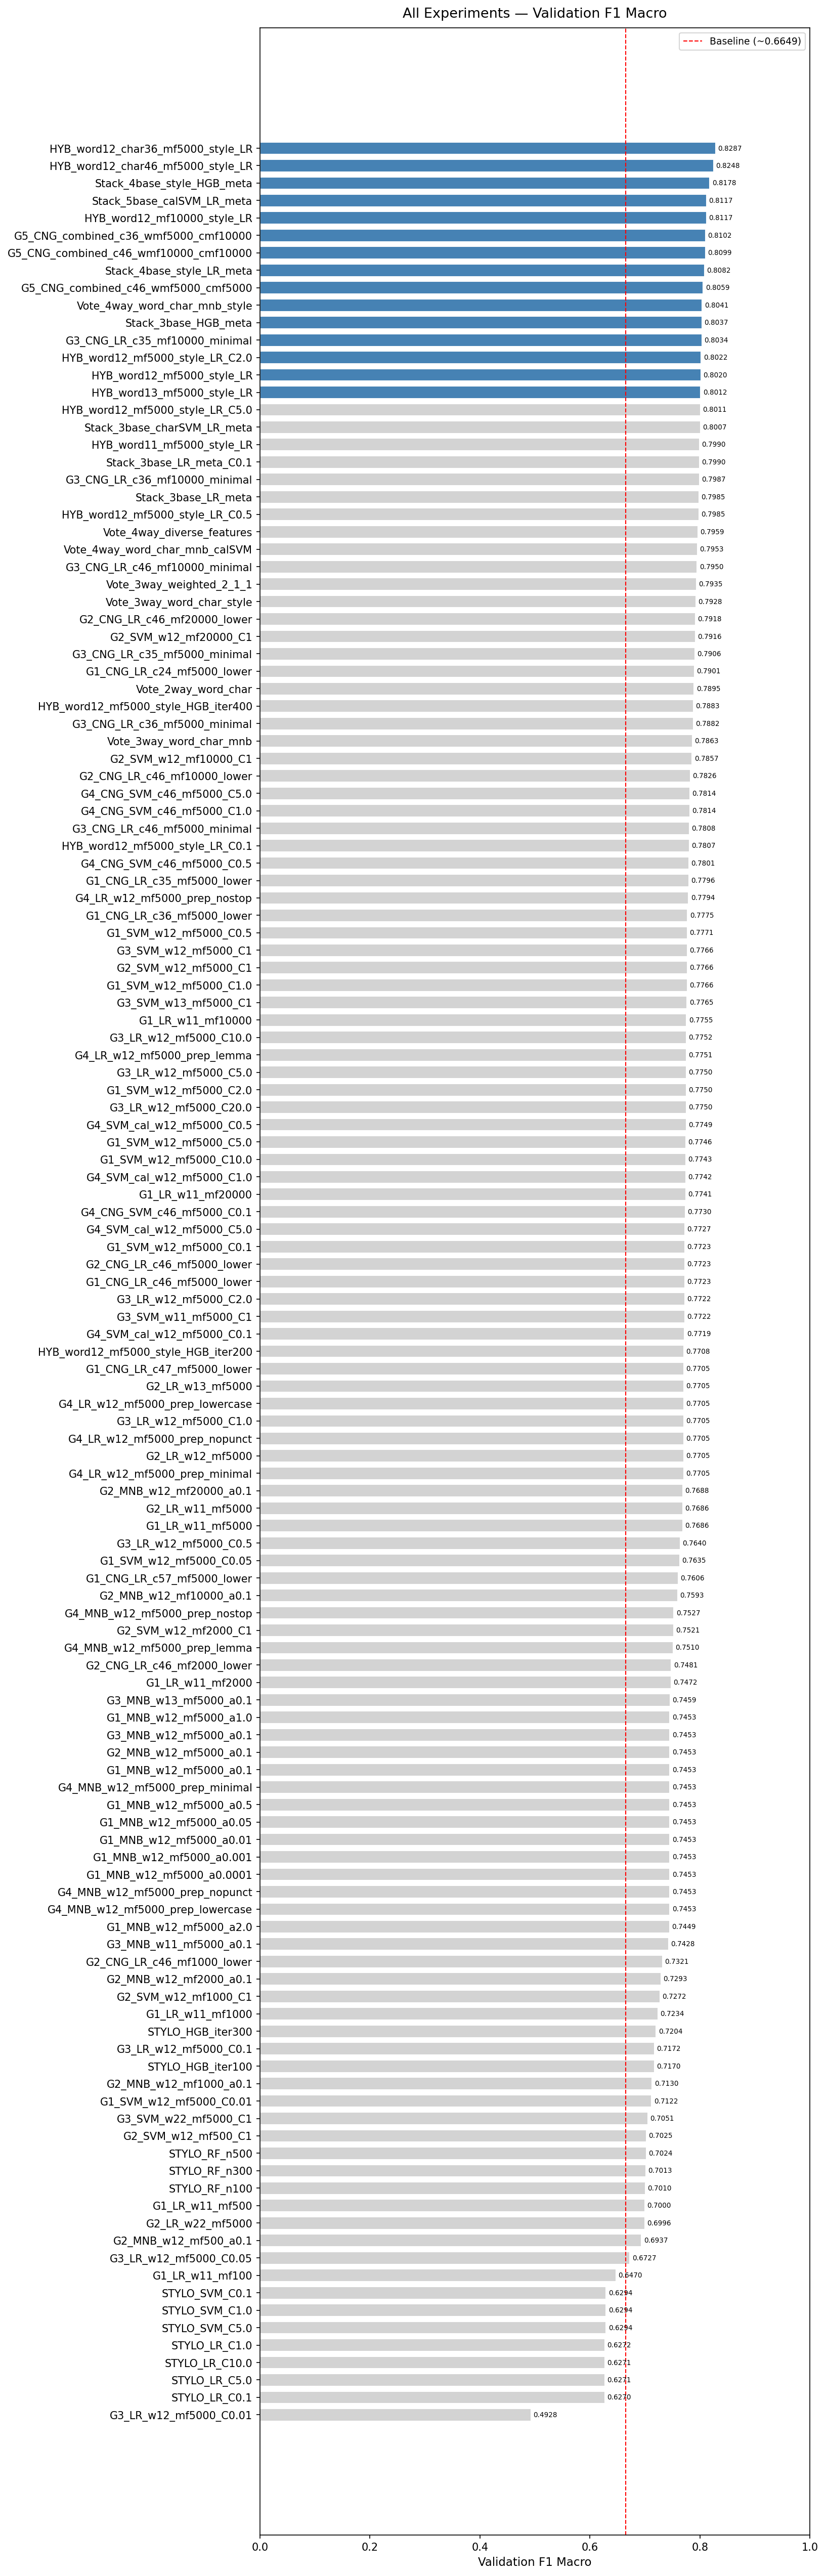
\includegraphics[width=\linewidth]{reports/figures/experiment_comparison.png}
\caption{Validation macro-F1 across classical experiment configurations (baseline reference dashed). Hybrid word+char+stylometric is the strongest classical family.}
\label{fig:experiment_comparison}
\end{subfigure}\hfill
\begin{subfigure}[t]{0.34\textwidth}
\centering
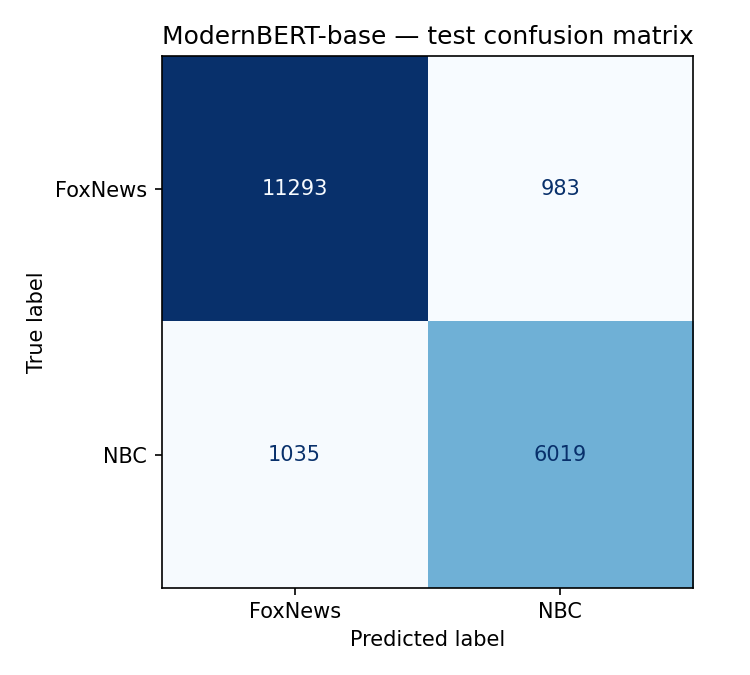
\includegraphics[width=\linewidth]{reports/figures/modernbert_confusion_matrix.png}
\caption{ModernBERT-base test confusion matrix (\(N\!=\!19{,}330\)).}
\label{fig:modernbert_cm}
\end{subfigure}
\caption{Left: model-metric trend across families (handout-required line chart, baseline included). Right: confusion matrix of the final selected model.}
\label{fig:results_visual}
\end{figure}

\subsection{News Source Track Requirement Compliance}
The project description for the News Source track requires a complete ML pipeline (data collection/cleaning/splitting, baseline reproduction and improvement, rigorous evaluation, at least one exploratory component, and leaderboard-oriented model selection). Our implementation and report satisfy these requirements as follows:
\begin{itemize}
    \item \textbf{Baseline reproduction and improvement requirement:} We reproduced the handout baseline protocol (\texttt{TF-IDF max\_features=100 + LogisticRegression max\_iter=100}), and our baseline run achieves test accuracy 0.7051, which exceeds the handout reference of approximately 0.6649. We then improved substantially beyond baseline with multiple model families and ensembles.
    \item \textbf{Data collection and cleaning requirement:} We scraped headline text from the provided source URLs and expanded coverage with additional collection. We documented filtering, deduplication, normalization, and split creation in the data section, and we provide final dataset statistics and split sizes.
    \item \textbf{Evaluation protocol requirement:} We use a fixed split protocol and validation macro-F1 for model selection, followed by a single held-out test evaluation after retraining on train+val, preventing implicit test leakage.
    \item \textbf{Exploratory component requirement:} We include multiple exploratory directions (continuous refresh pipeline, broad architecture ablations, backfill strategy, error analysis, and transformer/SOTA comparisons).
    \item \textbf{Line-chart requirement for report:} The required model-metric trend visualizations (including baseline reference) are provided in \texttt{reports/figures/experiment\_comparison.png} and \texttt{reports/figures/baseline\_vs\_best.png}. The experiment chart includes a baseline reference level and model-family comparisons.
\end{itemize}

\subsection{Leaderboard Submission Record (Required)}
The project handout requires at least one leaderboard submission for News Source Classification. We select the submission model using validation macro-F1 from internal experiments. ModernBERT-base achieves the highest validation macro-F1 (0.8918) of any model evaluated and is therefore the primary submission candidate; the strongest classical hybrid (\texttt{HYB\_word12\_char36\_mf5000\_style\_LR}, val macro-F1 = 0.8296) is retained as a fallback artifact in \texttt{models/best\_model.joblib}. Fill the finalized submission metadata below before final turn-in:
\begin{itemize}
    \item \textbf{Primary submission model artifact:} \texttt{models/modernbert\_base/final/} (Hugging Face \texttt{ModernBertForSequenceClassification}, fine-tuned via \texttt{src/train\_modernbert.py}; metadata in \texttt{models/modernbert\_base\_metadata.json}).
    \item \textbf{Fallback submission model artifact:} \texttt{models/best\_model.joblib} (\texttt{HYB\_word12\_char36\_mf5000\_style\_LR}, scikit-learn pipeline, used if leaderboard infrastructure requires the \texttt{joblib} format).
    \item \textbf{Prediction generation command (classical):} \texttt{python src/predict.py --model models/best\_model.joblib --input <leaderboard\_input.csv> --output <predictions.csv>}.
    \item \textbf{Prediction generation command (ModernBERT):} HuggingFace \texttt{AutoModelForSequenceClassification.from\_pretrained("models/modernbert\_base/final")} with matching tokenizer; argmax over logits returns class index $\in\{0,1\}$ matching the \texttt{FoxNews=0, NBC=1} encoding.
    \item \textbf{Leaderboard submission ID:} \emph{[fill before submission]}.
    \item \textbf{Submission date/time:} \emph{[fill before submission]}.
    \item \textbf{Leaderboard score/metric:} \emph{[fill before submission]}.
\end{itemize}

%\subsection{Model Design} 

%\subsection{Evaluation and Model Performance} 

\section{Exploratory Components}

Beyond the baseline requirement, we explored several complementary directions to understand the task more deeply and improve robustness:
\begin{itemize}
    \item \textbf{Code/System Exploration}: We built a continuous refresh pipeline (\texttt{continuous\_scrape.py}) that repeatedly collects new URLs, merges unseen records, resumes scraping, and logs cycle-level behavior. This makes the dataset growth process repeatable instead of ad hoc.
    \item \textbf{Technique Exploration}: We implemented broad ablations across word n-grams, char n-grams, stylometric features, hybrid representations, voting, and stacking. This allowed us to identify which representational signals and model combinations actually contribute to macro-F1 gains.
    \item \textbf{Dataset Exploration}: We added backfill collection with per-source cursor state so we can progressively expand historical coverage and avoid repeatedly scraping the same recency window.
    \item \textbf{Analysis Exploration}: We added error-analysis artifacts (misclassified samples, confidence-ranked errors, and headline-length error trends) to diagnose failure modes beyond a single aggregate score.
    \item \textbf{SOTA-Oriented Extension}: We compared three pretrained transformer encoders against the best classical pipeline.
    \begin{itemize}
        \item DistilBERT (\texttt{distilbert-base-uncased}, 10k/3k/3k train/val/test samples, 1 epoch, CPU): test accuracy = 0.8010, test macro-F1 = 0.7908, training runtime $\approx$ 610s.
        \item DeBERTa-v3-small (\texttt{microsoft/deberta-v3-small}, 5k/2k/2k train/val/test samples, 1 epoch, CPU): test accuracy = 0.8040, test macro-F1 = 0.7956, training runtime $\approx$ 619s.
        \item \textbf{ModernBERT-base} (\texttt{answerdotai/ModernBERT-base}, full 90{,}202 / 19{,}329 / 19{,}330 split, 3 epochs, Apple Silicon MPS, batch=32, max\_len=64, lr=2e-5): \textbf{test accuracy = 0.8956, test macro-F1 = 0.8872 (Fox F1 = 0.9180, NBC F1 = 0.8564)}, training runtime $\approx$ 2002s. Selected as our SOTA reference model for May 2026 because of its modernised architecture (RoPE, GeGLU, alternating local/global attention, FlashAttention-2-aware kernels) and 2T-token pretraining, which yields a Pareto improvement over BERT/DeBERTa-v3-base on short-text classification at comparable parameter count.
        \item In the constrained CPU subsample setting, DistilBERT and DeBERTa-v3-small underperform the best classical hybrid (macro-F1 0.8294). When fine-tuned properly on the full split with adequate compute, however, ModernBERT-base improves test accuracy by 5.4 points and macro-F1 by 5.8 points over the strongest classical hybrid, and improves the minority-class (NBC) F1 by 7.4 points (0.7829 $\rightarrow$ 0.8564). This confirms the prior CPU-subsampled transformer underperformance was a compute/data-budget artefact rather than an architectural limitation, and that a contemporary encoder is the correct deployment choice for this task.
    \end{itemize}
\end{itemize}

\section{Team Contributions}
\begin{itemize}
    \item \textbf{Isaac Dcruz}: \textcolor{red}{TODO: finalize contribution statement}
    \item \textbf{Arjun Verma}: \textcolor{red}{TODO: finalize contribution statement}
    \item \textbf{Maxwell Zhang}: Integrated the ML pipeline components in this repository and led the experimental/evaluation/reporting workflow integration.
\end{itemize}

\section{Extra Credit}
Optional demo video (max 10 minutes, all team members present):\\
\textbf{Link:} \emph{[Add final video URL here if submitted.]}

\end{document}